\documentclass[border=2pt]{standalone}
\usepackage{tikz}
\usetikzlibrary{arrows.meta,shapes.symbols}
\begin{document}
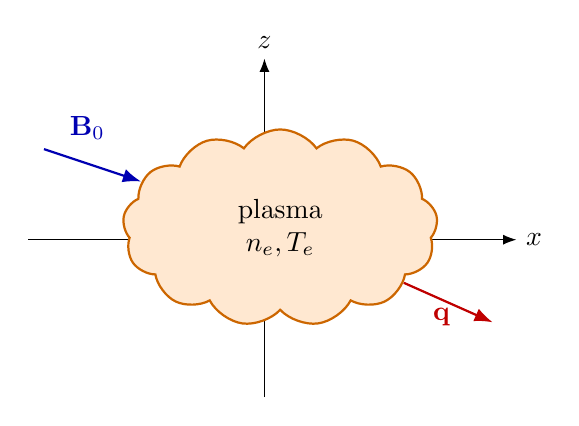
\begin{tikzpicture}[>=Latex]
  \draw[->] (-3,0) -- (3.2,0) node[right] {$x$};
  \draw[->] (0,-2) -- (0,2.3) node[above] {$z$};
  \node[cloud,cloud puffs=13,cloud puff arc=110,cloud ignores aspect,
        draw=orange!80!black,fill=orange!18,minimum width=40mm,minimum height=25mm,
        line width=0.8pt,align=center] (plasma) at (0.2,0.15) {plasma\\$n_e,T_e$};
  \draw[->,blue!70!black,thick] (-2.8,1.15) -- (plasma);
  \draw[->,red!75!black,thick] (plasma) -- (2.9,-1.05);
  \node[blue!70!black,above] at (-2.25,1.15) {$\mathbf B_0$};
  \node[red!75!black,below] at (2.25,-0.75) {$\mathbf q$};
\end{tikzpicture}
\end{document}
